%!TEX root = ../document.tex


\chapter{Das Nachfolgesystem ReEvent}
\label{ch:reevent}
%Da es sich die vorliegende Arbeit zum Ziel gemacht hat, eine auf die neue Veranstaltungsverwaltung ReEvent \index{ReEvent} zugeschnittene Suchlösung zu ermitteln, sollen im Folgenden die hierfür relevanten Grundlagen ReEvent betreffend geschaffen werden.

Nach \cite[S. 85]{Rupp.2014} ist es für den Prozess des Requirements Engineerings notwendig, den Systemkontext zu betrachten. Aus Sicht der Veranstaltungssuche stellt das Gesamtprojekt ReEvent einen unmittelbaren Nachbarn dar. Da die technischen Aspekte ReEvents Einfluss auf die Wahl der Suchlösung nehmen können, soll im Folgenden ein Überblick über grundlegende Eigenschaften des Systems vermittelt werden.

\section{Eine Veranstaltungsverwaltung}
\label{sec:reevent_about}

Wie bereits eingangs dargestellt, soll ReEvent das Altsystem INsite ablösen und die Funktion einer öffentlichen, kommunalen Veranstaltungsverwaltung übernehmen. Hierzu gehört die Eingabe neuer Veranstaltungsdaten aus diversen Quellen -- Vorschläge, die an die Redakteure per Email oder Webformular eingehen, ebenso wie automatisiert per Webservice übertragene Veranstaltungen des Ratsinformationssystems der Stadt.\footnote{ siehe \url{http://www4.ingolstadt.de/sessionnet/infobi.php}, das Ratsinformationssystem \emph{SessionNet} der Firma Somacos GmbH \& Co. KG.}

Veranstaltungen erhalten einen Namen, einen kurzen Beschreibungstext für eine Vorschau und einen optionalen, längeren Beschreibungstext. Des Weiteren können beliebige Dateien zu Veranstaltungen abgespeichert werden. Möglich sind beispielsweise Veranstaltungseinladungen im PDF- oder Microsoft Word"=Format, Videodateien oder Bilddateien.

Eingegebene Veranstaltungen können schließlich auf einer entsprechenden Website -- fortführend wird der Begriff des \emph{Frontends} verwendet -- veröffentlicht werden. Hier erhalten Benutzer einen Überblick über tagesaktuelle Veranstaltungen und können weiterführende Informationen über diese abrufen. Sowohl für das Frontend als auch das Backend soll eine Suchfunktion entstehen -- was den Kern dieser Arbeit darstellt.

Es sei des Weiteren erwähnt, dass sich ReEvent zum Zeitpunkt der Erstellung dieser Arbeit in Entwicklung befindet. Getroffene Aussagen über diese Software spiegeln demnach nur den aktuellen Stand wieder und müssen nicht auf die endgültige Version des Produktes zutreffen.

\paragraph{Backend} einer Webanwendung ist der zugangsbeschränkte Teil, in dem Konfiguration oder redaktionelle Aufgaben durchgeführt werden. In ReEvent werden im Backend Veranstaltungen eingepflegt und bearbeitet.

\paragraph{Frontend} wiederum ist eine Menge von Seiten, welche prinzipiell öffentlich zugänglich sind. In ReEvent sollen Veranstaltungen in einem frei zugänglichen Kalender über das Internet aufgerufen werden können. Wird für manche oder alle Teile des Frontends ebenfalls ein Benutzerkonto benötigt -- beispielsweise für ein Kundenkonto in einem Onlineshop-System -- so wird dies als \emph{Frontend-Benutzer} bezeichnet.

\section{Auswahl der zugrundeliegenden Plattform}

Zu Beginn der Entwicklung von ReEvent steht die Frage nach der zu verwendenden Programmiersprache, beziehungsweise nach einem darauf aufbauenden Framework. Hierfür bieten sich mehrere Möglichkeiten an, welche teils schon in vorangegangen Projekten bei response eingesetzt wurden.

\subsection{Adobe ColdFusion}

Bereits die bestehende Anwendung INsite wurde auf Basis des Application Servers \emph{Adobe\,ColdFusion} entwickelt. Die ColdFusion"=Plattform bietet eine Implementierung der Webprogrammiersprache \emph{ColdFusion Markup Language} -- kurz CFML -- an \cite[S. 8]{Forta.2010}.\footnote{ColdFusion und CFML werden in der Literatur häufig synonym verwendet}

Neben INsite wurden auch weitere Teilbereiche des Webauftritts der Stadt Ingolstadt mit ColdFusion erstellt: Beispiele hierfür stellen der Newsletterversand\footnote{ siehe \url{http://www2.ingolstadt.de/newslet
ter}} und die Seiten des Stadttheaters\footnote{ siehe \url{http://theater.ingolstadt.de/}} dar. Somit kann response auf einen aufgebauten Erfahrungsschatz zurückgreifen, was durchaus für die Verwendung von ColdFusion für die Entwicklung von ReEvent spricht.

Im Gegensatz zu vergleichbaren Programmiersprachen ist Adobe ColdFusion jedoch nicht frei verfügbar und muss von Adobe kostenpflichtig lizenziert werden. Die \emph{Standard}-Edition von ColdFusion 11 wird für \numprint{1783,81}\,€ angeboten. Auch wenn dies prinzipiell nur ein einmaliger Posten ist, müssen die Upgradegebühren auf die nächste Versionsnummer ebenfalls mit eingeplant werden.\footnote{Preisangabe inklusive Mehrwertsteuer, Stand 06.09.2015, vergleiche \url{http://www.adobe.com/de/products/coldfusion-family.html}}\footnote{das Upgrade von ColdFusion 10 Standard auf die Version 11 schlägt derzeit mit \numprint{891,31}\,€ zu Buche} Ein Upgrade kann nach Auslaufen des Supportzeitrahmens einer Version zwingend notwendig werden, da keine weiteren Sicherheitsupdates ausgeliefert werden. Alternativ zu Adobe ColdFusion existieren auch freie Implementierungen der CFML, wie beispielsweise Railo \cite[Abschnitt \enquote{Inexpensive and free}]{Drew.2011}. Für die Stadt Ingolstadt spielt dieser Punkt nur eine untergeordnete Rolle, da aufgrund bestehender Applikationen in jedem Fall eine Lizenz für Adobe ColdFusion vorliegt. Allerdings würde sich mit ReEvent als ColdFusion"=Applikation eine weitere Abhängigkeit im Falle eines Systemwechsels aufbauen.

Ein weiteres Argument gegen die Verwendung von ColdFusion stellt die stetig sinkende Verbreitung der Programmiersprache dar. Beispielsweise ist die CFML nicht länger im TIOBE Index enthalten \cite{TIOBESoftwareBV.2015}. Der nicht unumstrittene Index ermittelt die Trefferzahlen für die Suchanfrage \texttt{+"{}<language> programming"{}} in 25 verschiedenen Suchmaschinen und leitet daraus ein Popularitätsranking ab \cite{MengeSonnentag.2015}. Aufgeführt werden bis zu 100 Sprachen -- derzeit ohne ColdFusion.\footnote{Stand 22.10.2015, TIOBE Index Oktober}
Auch die Statistik in Abbildung \ref{fig:w3tech.languages} von W3Techs weist für ColdFusion einen Marktanteil von lediglich 0.7\% Prozent vor.
Während die Verbreitung einer Programmiersprache selbst nichts über ihre Qualität oder Eignung für ein spezifisches Projekt aussagt, so sind die daraus entstehenden Folgen durchaus legitime Entscheidungskriterien. So ist über die vergangen Jahre ein Sterben einiger großer auf ColdFusion aufbauender Frameworks zu beobachten. Tabelle \ref{tab:ColdFusion.Frameworks} listet frei verfügbare Frameworks für ColdFusion auf. Lediglich zwei der Einträge werden derzeit aktiv weiterentwickelt.\footnote{Stand 25.10.2015} Entsprechend ist die Kompatibilität dieser Frameworks mit kommenden Versionen von Adobe ColdFusion oder Railo nicht sichergestellt. ORM"=Bestandteile der Frameworks werden ebenfalls nicht länger an neue Versionen der gängigen Datenbanksysteme angepasst. Somit ist fraglich, ob die Verwendung der ColdFusion"=Plattform als zukunftssicher bezeichnet werden kann.


\subsection{Flow und Neos CMS}

Neben Adobe ColdFusion nutzt response auch das Content Management System TYPO3 sowohl für Kundenprojekte als auch für die firmeneigene Homepage \cite{responseinformationsdesigngmbh&co.kg.}. Zusätzlich zur Verwaltung von einfachen Webseiteninhalten wie Text und Bild bietet das PHP-basierte TYPO3 auch die Möglichkeit, das System durch selbstgeschriebene Erweiterungen zu ergänzen \cite[S. IX]{Rau.2014}. Diese \emph{Extensions} können zudem Funktionen des Grundsystems nutzen -- wie beispielsweise die Benutzerverwaltung. Aufgrund dessen stellt TYPO3 eine mögliche Entwicklungsplattform für ReEvent dar.

Hierbei ist allerdings eine grundsätzliche Entscheidung zu treffen: Zum aktuellen Zeitpunkt existieren zwei Entwicklungsstränge des CMS. Zur Entwicklung der Version 5 von TYPO3 wurde das System von Grund auf neugeschrieben. Die neue Version sollte auf einem eigens hierfür programmierten PHP"=Framework namens FLOW3 basieren. Im weiteren Verlauf wurde jedoch entschieden, das neue System als eigenständiges Produkt weiterzuentwickeln \cite[S. X]{Rau.2014}. Die beiden Projekte divergierten weiter, bis sie sich schließlich voneinander trennten. Seit Herbst 2015 ist das inzwischen umbenannte \emph{Neos CMS} von der TYPO3 Association losgelöst, auch der Name des Frameworks wurde zu \emph{Flow} geändert \cite{NeosCMS.2015b}. Das ursprüngliche TYPO3 wird nun als TYPO3 CMS fortgeführt. Um Verwechslungen mit Neos zu vermeiden hat man die folgende Version von TYPO3 CMS auf die Versionsnummer 6 angehoben \cite[S. XIII]{Rau.2014}.

Flow stellt ein nach dem \emph{Model-View-Controller} Pattern funktionierendes Webframework dar, welches mit ORM, AOP, Dependency Injection und Templating viele moderne Features mit sich bringt. Als objektrelationaler Mapper wird \emph{Doctrine} eingesetzt, die Views werden von der Templating Engine \emph{Fluid} gerendert.

Wie bereits eingangs erläutert, kann TYPO3 durch Extensions um benötigte Funktionen erweitert werden. Für TYPO3 CMS gibt es frei verfügbare Erweiterungen, wie das \emph{powermail}-Plugin zum Versand von Newsletter-Mails. Diese können vom offiziellen Extension Repository\footnote{siehe \url{https://typo3.org/extensions/repository/}} bezogen werden, welches derzeit\footnote{Stand 25.12.2015} \numprint{1316} Plugins bereitstellt. Wenn auch geplant, so gibt es derzeit kein vergleichbares Angebot für Neos CMS. Die offizielle Webseite von Neos geht von \enquote{ein paar hundert} verfügbaren Extensions aus und verweist auf die Seite \url{https://packagist.org/} \cite{NeosCMS.2015}. Die geringere und schlechter organisierte Verfügbarkeit von Erweiterungen schränkt Neos im Vergleich zu TYPO3 CMS ein, insbesondere beim Aufbau komplexerer Webseiten könnte sich ein reiches Angebot an Plugins als hilfreich erweisen.

Das ursprüngliche TYPO3 CMS hat den Ruf eines \enquote{komplexe[n] und schwer zu erlernende[n] Programm[es]} \cite[S. X]{Bielitza.2011}. Dies ist zum Teil auch dem schieren Umfang der als Enterprise-CMS titulierten Anwendung geschuldet: Mehrsprachigkeit, Content-Review und Benutzerverwaltung sind Funktionen, die eher in größeren Webauftritten notwendig sind. Einen Schritt in die richtige Richtung machte Neos mit einer starken Überarbeitung des Benutzerinterfaces: Als auffälligstes Merkmal wird die Frontendseite direkt in das Backend eingebettet, Inhalte können \emph{inline} bearbeitet werden. Dadurch erhält der Benutzer bereits bei der Eingabe der Änderung ein Feedback über die Auswirkung auf die ausgegebene Seite.

\begin{figure}[ht!]
\begin{margincap}
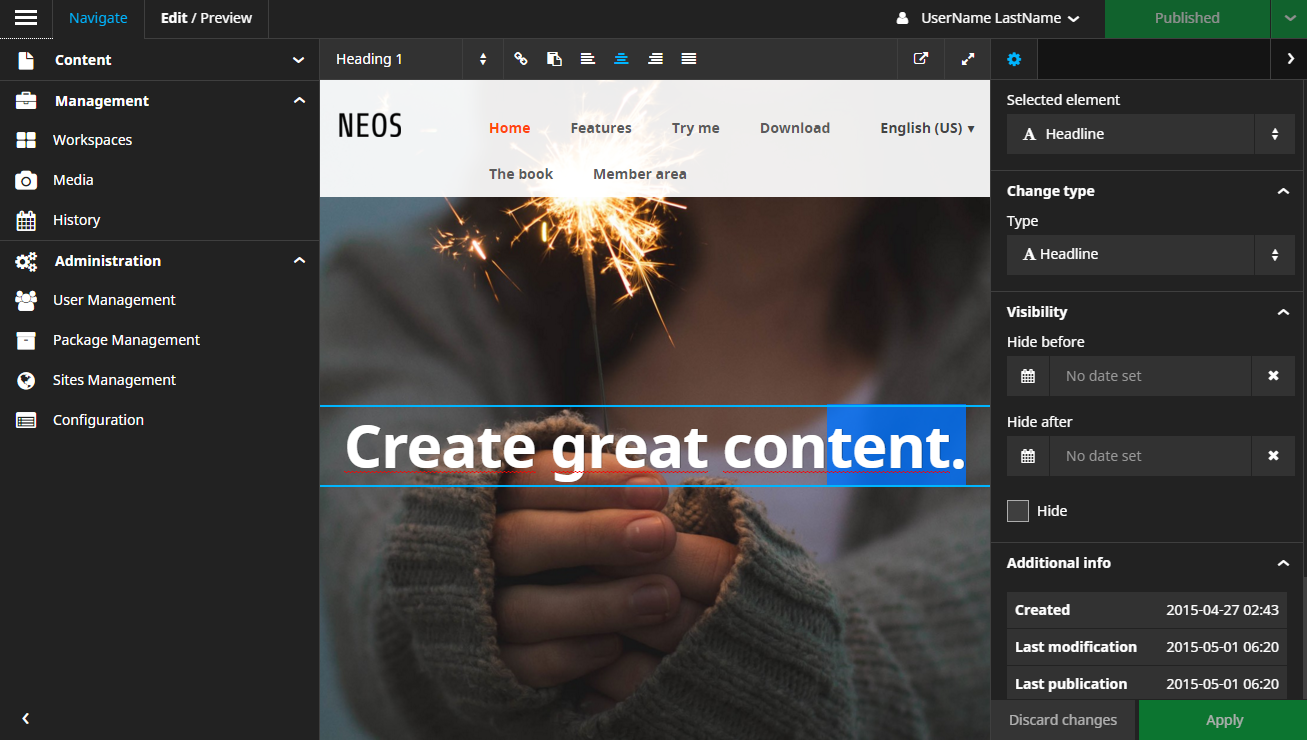
\includegraphics[width=\textwidth]{screenshot_neos_cms.png}
\caption[Neos CMS Backend]{Backend von Neos CMS, gezeigt wird der Inline"=Texteditor. Das Backend ist responsive aufgebaut, über das Menü links oben kann auf installierte Packages zugegriffen werden -- wie auch auf ReEvent.}
\label{img:neos_backend_screenshot}
\end{margincap}
\end{figure}

Die Auftrennung in zwei Entwicklungsstränge bringt nicht nur Positives mit sich: Finanzielle Mittel verbleiben bei der TYPO3 Association, Neos CMS ist daher teils auf Spenden angewiesen \cite{NeosCMS.2015b}. Neben der monetären Aufteilung bedeutet die gleichzeitige Pflege zweier Produkte auch eine verkleinerte Zahl an Entwicklern für ein einzelnes Projekt. Auch die Anwender werden durch die Konkurrenzsituation zwischen den beiden Projekten in zwei Lager getrennt, was einer Schwächung der Community gleichkommen dürfte.

\subsection{Alternativen}

Adobe ColdFusion und Neos CMS sind nicht die einzigen Lösungen, die für ein Projekt wie ReEvent in Frage kommen.

\subsubsection{symfony}
symfony ist wie auch Flow ein Web-Framework auf Basis von PHP. Mit einem ersten Release im Dezember 2005 ist es vergleichsweise länger am Markt als das 2011 veröffentlichte Flow \cite[S. 21]{Potencier.}. Wenn auch nicht auf den ersten Blick ersichtlich, so bestehen dennoch Zusammenhänge zwischen den beiden Frameworks: So verwenden beide Doctrine als ORM. Auch nutzt Flow einige Packages von symfony, wie beispielsweise zum Parsen von Konfigurationsdateien.\footnote{ siehe composer.json von Flow, \url{https://github.com/neos/flow-development-collection/blob/893358e66fc3e3e0fe4439db18564568298ab6a6/composer.json}} Anders als Flow unterstützt symfony jedoch keine aspektorientierte Programmierung.

\subsubsection{Ruby on Rails}

Bereits seit 2004 gibt es mit dem auf der Skriptsprache Ruby basierenden \emph{Ruby on Rails} einen weiteren Vertreter der Webframeworks \cite[S. 1]{Orsini.2007}. Anders als Doctrine unter Flow setzt Rails auf das \emph{ActiveRecord}-Pattern zur Speicherung und Bearbeitung von Objekten in der Datenbank. Während Doctrine mit einfachen PHP-Objekten arbeitet, welche über Repositories in die Datenbank übertragen werden, verfügt unter Rails jede Model-Klasse über Funktionen wie \mintinline{rb}{save} oder \mintinline{rb}{delete}.

Der Einfluss von Ruby on Rails auf jüngere Frameworks ist durchaus gegeben: Das ColdFusion-Framework CFWheels -- eines der beiden, die noch aktiv weiterentwickelt werden -- ist der Struktur nach Ruby on Rails nachempfunden.

Bisher konnte das Entwicklerteam bei response weder mit der Skriptsprache noch mit dem Framework Erfahrungen sammeln, was vermutlich in einer hohen Einarbeitungsdauer resultieren würde.

\subsubsection{Andere erweiterbare CMS}

Neben TYPO3 CMS und Neos CMS existieren auch weitere Content Management Systeme, deren Funktionsumfang durch Erweiterungen ergänzt werden kann. Als Beispiele hierfür sind WordPress oder Joomla zu nennen -- beide basieren ebenfalls auf PHP.

Laut einer weiteren Studie von W3Techs nutzen 25,7\,\% aller Webseiten die Blogsoftware WordPress \cite{W3Techs.2016} -- was möglicherweise auch der einfachen Bedienung geschuldet ist. Prinzipiell ist WordPress eher darauf ausgelegt, auch von Anwendern mit geringerem technischem Hintergrund eingerichtet und verwendet zu werden. So wirbt WordPress auf der offiziellen HomePage\footnote{siehe \url{https://wordpress.org/}, Stand 11.01.2016} mit einer \enquote{5-minute installation}. Auf der technischen Seite fällt allerdings ein Unterschied zu beispielsweise Neos CMS auf: Als Datenbank wird offiziell nur MySQL unterstützt, Ports zu PostgreSQL wurden nicht weitergeführt.\footnote{siehe \url{https://codex.wordpress.org/Using\_Alternative\_Databases}}

Es sei des Weiteren angemerkt, dass CMS-Funktionen nicht den entscheidenden Faktor für die Systementwicklung von ReEvent darstellen. Ein CMS stellt üblicherweise Komponenten wie eine Benutzer- oder Mediendatenverwaltung bereit. Auch wenn diese in ReEvent möglicherweise wiederverwendet werden könnten, so sollte dennoch ein zugrundeliegendes Framework die Entwicklung von ReEvent maximal unterstützen. Ausgehend von den Dokumentationen von WordPress und Joomla geht nicht hervor, dass die zur Verfügung gestellte Plattform in ihrem Funktionsumfang mit Flow mithalten kann.\footnote{siehe \url{http://codex.wordpress.org/Writing\_a\_Plugin} und \url{https://docs.joomla.org/J3.x:Developing\_an\_MVC\_Component/Developing\_a\_Basic\_Component}}


\subsection{Fazit}
Selbstverständlich ist die hier vorgestellte Auswahl an Möglichkeiten nicht erschöpfend. Mit diversen Java-Webframeworks, ASP .Net, Drupal oder node.js gibt es noch eine Vielzahl weiterer aktueller Systeme, die prinzipiell für die Entwicklung von ReEvent in Frage kommen. Die präsentierten Varianten bilden jedoch einen groben Querschnitt über die am Markt befindlichen Konkurrenten zu Flow und ColdFusion stehen auch stellvertretend für nicht miteinbezogene Alternativen.

Basierend auf der Annahme, dass jene Programmiersprache am geeignetsten ist, mit welcher das Entwicklerteam am besten umgehen kann, ist PHP durchaus eine schlüssige Wahl. Sowohl Flow als auch andere PHP-Frameworks wurden jedoch in keinen früheren Projekten bei response eingesetzt.

Derzeit\footnote{Stand 10.01.2016} wird seit beinahe einem Jahr unter der Kombination von Flow und Neos CMS an ReEvent gearbeitet. Die Wahl erfolgte unter anderem unter dem Gesichtspunkt der Vorreiterrolle als Erster eine Veranstaltungsverwaltung für Neos CMS anbieten zu können. In diesem Zusammenhang offenbarten sich auch einige Kritikpunkte an Flow -- beispielsweise die nach wie vor unvollständige Dokumentation\footnote{vergleiche \url{http://flowframework.readthedocs.org/en/stable/TheDefinitiveGuide/index.html}} oder Caching-Probleme und lange Ladezeiten nach Änderungen von PHP-Quelltext. Somit wäre es möglicherweise vorteilhaft gewesen, auf ein etablierteres Framework wie symfony zu setzen.

Insbesondere da mit der Entwicklung von ReEvent auf Basis von Neos CMS und Flow bereits begonnen wurde, wird diese Auswahl für die kommenden Inhalte dieser Arbeit als gesetzt angenommen.

\section{Wahl der Datenbanklösung}
\label{sec:reevent.database}

Die von ReEvent verwalteten Daten -- prinzipiell PHP-Objekte des Flow"=Frameworks -- werden in einer Datenbank abgespeichert. Das Anlegen, Lesen, Aktualisieren und Löschen\footnote{CRUD - create, read, update und delete sind die gängigen Operationen einer Anwendung} dieser Objekte wird vom ORM-System \emph{Doctrine} in SQL-Anfragen umgewandelt. Da verschiedene Datenbanksysteme die SQL"=Standards nur teilweise oder leicht unterschiedlich implementieren, greift Doctrine auf die zugrundeliegende Datenbank über eine \emph{Database Abstraction Layer} zu, welche -- wie der Name sagt -- den Zugriff von der verwendeten Datenbank abstrahiert. Doctrine kann derzeit folgende Datenbanksysteme ansprechen \cite{TheDoctrineProject.2015}.

\begin{multicols}{2}
\begin{itemize}
	\item MySQL
	\item PostgreSQL
	\item Microsoft SQL Server (MSSQL)
	\item Oracle
	\item Sybase SQL Anywhere
	\item SQLite
	\item Drizzle
\end{itemize}
\end{multicols}

response hatte zuvor in anderen Projekten die Stadt Ingolstadt betreffend sowohl MySQL als auch das Pendant von Microsoft eingesetzt. Einem LAMP-Stack\footnote{Ein LAMP-Stack bezeichnet eine in der Webentwicklung häufig eingesetzte Kombination aus Linux, Apache Webserver, MySQL Datenbank und PHP} entsprechend wird ReEvent derzeit mit MySQL entwickelt. Ein Test mit dem aktuellen Entwicklungsstand von ReEvent ergab, dass die Datenbank problemlos durch PostgreSQL ersetzt werden könnte.

Neben den hier aufgelisteten relationalen Datenbanken gab es bereits Ansätze, eine dokumentenbasierte Datenbank wie \emph{CouchDB} in das Framework Flow zu integrieren. Diese wurde jedoch scheinbar nicht fortgeführt.\footnote{siehe \url{https://github.com/radmiraal/Radmiraal.CouchDB}} Derzeit verwaltet INsite circa \numprint{45000} Veranstaltungen und damit eine ähnliche Anzahl von Zeilen in der zugehörigen relationalen Datenbank.\footnote{siehe Statistik \ref{fig:events_per_year_insite}} Probleme hinsichtlich Auslastung der Datenbank sind zum aktuellen Zeitpunkt nicht aufgetreten. Da die Zahl der Datensätze in Flow vermutlich ähnlich dimensioniert sein wird, ist die Einführung einer NoSQL"=Datenbank hinsichtlich besserer Verteilbarkeit und Verfügbarkeit nicht notwendig.\footnote{Die im Folgenden vorgestellten Konzepte verlangen es teilweise, dass von einer Veranstaltung mehrere Versionen persistiert werden. Abhängig davon, wie stark diese Funkionen genutzt werden, könnte auch die Zahl der Datensätze ansteigen.} Dennoch sollte man die Möglichkeit eines Umstiegs auf eine NoSQL-Lösung nicht völlig außer Acht lassen. Aufgrund der starken Abhängigkeit des Flow-Frameworks und des geschriebenen Quellcodes zu Doctrine würde ein solcher Umstieg zu einem späteren Zeitpunkt jedoch großen Aufwand erfordern.

Was Doctrine schließlich noch im Vergleich zu ORM-Lösungen anderer Programmiersprachen\footnote{wie beispielsweise Hibernate unter Java} abhebt, ist die Fähigkeit aus den geschriebenen PHP-Klassen heraus automatisch die Tabellenstruktur der Datenbank anzulegen. Werden Änderungen am Klassenmodell vorgenommen, so kann SQL"=Code generiert werden\footnote{sogenannte Migration-Skripte}, der die Datenbanktabellen wieder entsprechend anpasst.

\section{Ansätze zur Modellierung der Mehrsprachigkeit}
\label{sec:ReEvent:MultiLanguage}

Anders als INsite soll ReEvent grundsätzlich auf Mehrsprachigkeit ausgelegt sein. Dies betrifft zum einen die Benutzeroberfläche, welche spezifisch für den User lokalisiert werden soll. Da jedoch städtische Veranstaltungen durchaus für ein internationales und multikulturelles Publikum von Interesse sind, sollte auch eine Übersetzung einzelner Veranstaltungen in ReEvent möglich sein. Ein relevantes Beispiel hierfür stellen Ereignisse im Rahmen der Ingolstädter Städtepartnerschaften dar.

Während die Internationalisierung statischer Oberflächen ein gängiges Feature aktueller Web"=Frameworks ist -- Flow setzt an dieser Stelle auf Übersetzungskataloge im xliff-Format auf welche über die eingebaute Template"=Engine Fluid zugegriffen werden kann \cite[S. 278, 280f]{TheNeosTeam.2015} -- fehlt meist die Möglichkeit, eingepflegte Inhalte zu übersetzen. Dies ist auch beim PHP-Framework Flow der Fall.

Dementsprechend stellt sich die Frage der Umsetzung der Mehrsprachigkeit, welche im Folgenden thematisiert wird.

\subsection{Verwendung des Content Dimension"=Konzepts von Neos CMS}
\label{sec:ReEvent.Language.Nodes}

\begin{center}
\parbox{0.9\textwidth}{
\itshape
\small
Die in diesem Abschnitt \ref{sec:ReEvent.Language.Nodes} vorgestellten Konzepte wurden von Mitarbeitern der Firma response ausgearbeitet und werden an dieser Stelle lediglich als Hintergrundinformation mit angegeben.
}
\end{center}

Das Content Management System Neos ermöglicht Übersetzung von Inhalten auf Basis von \emph{Nodes} genannten Strukturen. Jeder Inhalt einer durch Neos verwalteten Seite -- beispielsweise Textblöcke oder Grafiken -- wird durch einen Node repräsentiert \cite[S. 15f]{TheNeosTeam.2015b}. Welche Attribute ein Node beinhaltet, ist abhängig vom \emph{Node Type} dieses Nodes. Node Types stellen \enquote{Baupläne} für Nodes dar, sie verhalten sich somit ähnlich wie Klassen zu Objekten \cite[S. 15f]{TheNeosTeam.2015b}.

Zur Übersetzung lässt sich in Neos das generische Konzept von \emph{Content Dimensions} nutzen. Eine Content Dimension entspricht einer Möglichkeit, für einen Node Inhaltsvarianten anzulegen. Wurde beispielsweise eine Content Dimension \emph{Sprache} definiert, so können für einzelne Sprachen $\{en\_GB,de\}$ übersetzte Varianten des Nodes hinterlegt werden.

Content Dimensions lassen sich zudem miteinander verbinden: Angenommen, es wird  neben \emph{Sprache} auch \emph{Altersgruppe} und \emph{Ausgabe"=Gerätetyp} erzeugt, so können für alle möglichen Kombinationen personalisierte und angepasste Inhalte eines Nodes definiert werden \cite[S. 60]{TheNeosTeam.2015b}.


\begin{figure}[ht!]
\begin{margincap}
\centering
\tdplotsetmaincoords{60}{110}
\begin{tikzpicture}[tdplot_main_coords]
\draw[thick,->] (0,0,0) -- (4,0,0) node[anchor=north east]{\itshape Ausgabe"=Ger"atetyp};
\draw[thick,->] (0,0,0) -- (0,4,0) node[anchor=north west]{\itshape Altersgruppe};
\draw[thick,->] (0,0,0) -- (0,0,4) node[anchor=south]{\itshape Sprache};

\draw (0,0,1.5) -- (0,-0.25,1.5) node[anchor=south east]{de};
\draw (0,0,3) -- (0,-0.25,3) node[anchor=south east]{en\_GB};

\draw (1.5,0,0) -- (1.5,-0.25,0) node[anchor=south east]{mobil};
\draw (3,0,0) -- (3,-0.25,0) node[anchor=south east]{Desktop};

\draw (0,1.5,0) -- (-0.25,1.5,0) node[anchor=south west]{Kinder};
\draw (0,3,0) -- (-0.25,3,0) node[anchor=south west]{Erwachsene};

\draw[ultra thick,->,MyDarkBlue] (0,0,0) -- (1.5,0,0);
\draw[ultra thick,->,MyDarkBlue] (1.5,0,0) -- (1.5,1.5,0);
\draw[ultra thick,->,MyDarkBlue] (1.5,1.5,0) -- (1.5,1.5,3);

%\draw[thick] (1.7,1.5,3) -- (1.3,1.5,3);
%\draw[thick] (1.5,1.6,2.9) -- (1.5,1.4,3.1);

\end{tikzpicture}
\caption[Abstrakte Darstellung des Content Dimensions Konzepts aus Neos CMS]{Content Dimensions können in Neos miteinander kombiniert werden -- die Grafik zeigt eine mögliche Auswahl nach Sprache, Altersgruppe und Gerätetyp für die Ausgabe}
\label{img:ContentDimensions}
\end{margincap}
\end{figure}

%TODO Klar machen, weiter oben, dass ReEvent backend modul von Flow wird -- eventuell im Fazit
Da ReEvent als Backend"=Modul für Neos konzipiert wurde, wirft dies die Frage auf, ob sich Content Dimensions für die Mehrsprachigkeit in ReEvent verwenden lassen.

Dies verlangt es, den übersetzbaren Teil einer Klasse vom sprachinvarianten Part zu trennen. Beispielsweise verbleiben Relationen und Zahlenwerte wie GPS-Koordinaten in der ursprünglichen Klasse, während Benennungen oder Beschreibungen in einen Node verschoben werden.

\begin{figure}[ht!]
\begin{margincap}
\centering
\begin{tikzpicture}
\umlclass[x=1,y=0]{GeoLocation}{latitude : float \\ longitude : float \\ name : string \\ description : string}{}
\node[font=\Huge] () at ($(GeoLocation.east) +(1.3,0)$){$\Rightarrow$};
\umlclass[x=7,y=1.5]{GeoLocation}{latitude : float \\ longitude : float}{}
\umlclass[x=7,y=-1.5,type=Node]{GeoLocationNode}{name : string \\ description : string}{}

\draw[->, thick] (GeoLocation.east) -| ( $(GeoLocation.east) +(1,0)$ ) |- (GeoLocationNode.east);

\draw plot coordinates{ (GeoLocation.east)} node[above right] {1};
\draw plot coordinates{ (GeoLocationNode.east)} node[above right] {1..*};
\end{tikzpicture}
\caption{Auslagerung des übersetzbaren Teils einer Klasse in einen Neos Node am Beispiel der Klasse \texttt{GeoLocation}}
\label{img:ClassToNode}
\end{margincap}
\end{figure}

Über Getter- und Setter"=Funktionen kann anschließend transparent auf die im Node gespeicherten Daten zugegriffen werden.\footnote{\textit{information hiding} oder Geheimnisprinzip, vgl. \cite[S. 26]{Balzert.1999}}

Nachteilig an diesem Vorgehen ist die Art, in welcher Nodes in der Datenbank abgespeichert werden. Da Nodes vom Prinzip her generisch angelegt sind, werden die Attribute eines Nodes nicht in einer Klasse, sondern in externen Konfigurationsdateien definiert \cite[S. 16]{TheNeosTeam.2015b}.\footnote{eine entsprechende Definition in einer Konfigurationsdatei heißt \emph{NodeType}} Dies führt allerdings dazu, dass dem ORM-Framework die Attribute eines speziellen Nodes nicht bekannt sind, sie werden daher als JSON kodiert und in der Datenbank abgespeichert.\footnote{vgl. \url{https://github.com/neos/typo3cr/blob/d4dd8bcab165b7bd7248093e444f89ce49a751a0/Classes/TYPO3/TYPO3CR/Domain/Model/AbstractNodeData.php\#L35}, Zeile 35} Im Umkehrschluss bedeutet dies, dass das ORM auch beim Zugriff auf die Inhalte des Nodes eingeschränkt ist: Funktionen zur Filterung oder Sortierung, welche vom ORM für normale PHP"=Objekte angeboten werden, können im Falle von Nodes nicht auf die als JSON gespeicherten Daten zugreifen. Entsprechend müssten diese Funktionen außerhalb der Datenbank nachimplementiert werden.\footnote{Es sei darauf hingewiesen, dass gängige Datenbanksysteme wie MySQL, PostgreSQL und MSSQL einen Datentyp für JSON Dokumente anbieten. Dieser wird allerdings lediglich im Falle von PostgreSQL durch Doctrine verwendet \cite[vgl. 8.2 Mapping Types]{TheDoctrineProject.}.}

\subsection{Ersetzung einzelner Attribute durch übersetzbare Objekte}

Alternativ kann jedes einzelne Attribut, welches übersetzbar sein soll, in ein eigenes Objekt ausgelagert werden. Dieses Objekt stellt einen Container dar, welcher für einzelne Sprachen eine Variante des Attributs beinhaltet. Eine mögliche Modellierung hiervon zeigt die Grafik \ref{img:TranslatableGeoLocation}.

\begin{figure}[ht!]
	\begin{margincap}
	\centering
		\begin{tikzpicture}
		\umlclass[x=0,y=1.5]{GeoLocation}{latitude : float \\ longitude : float}{}

		\umlclass[x=8,y=-1]{Translatable}{}{+ get(lanuage : LanguageType) \\ + set(lanuage : LanguageType)}
		\umlclass[x=8,y=2]{Translation}{content : string \\ language : LanguageType}{}

		\draw[->, thick] (GeoLocation.east) -| ( $(Translatable.west) +(-2,0)$ ) |- (Translatable.west);
		\draw plot coordinates{(GeoLocation.east)} node[above right] {1};
		\draw plot coordinates{( $(Translatable.west) +(-2,0.5)$ )} node[right] {name};
		\draw plot coordinates{(Translatable.west)} node[above left] {1};

		\draw[->, thick] ( $(GeoLocation.east) + (0,-0.5)$) -| ( $(Translatable.west) +(-2.5,-0.5)$ ) |-  ( $(Translatable.west) + (0,-0.5)$);
		\draw plot coordinates{ ( $(GeoLocation.east) + (0,-0.5)$)} node[below right] {1};
		\draw plot coordinates{( $(Translatable.west) +(-2.0,-0.6)$ )} node[below] {description};
		\draw plot coordinates{($(Translatable.west) + (0,-0.5)$)} node[below left] {1};

		\draw[<-, thick] (Translation.east) -| ( $(Translatable.east) +(0.5,0)$ ) |- (Translatable.east);
		\draw plot coordinates{ ( Translatable.east)} node[above right] {1};
		\draw plot coordinates{ ( Translation.east)} node[above right] {0..*};
		\end{tikzpicture}
		\caption[Translatable-Objekte am Beispiel der Klasse GeoLocation]{Transferierung von übersetzbaren Attributen in eine \texttt{Translatable} Klasse, welche in Abhängigkeit von der übergeben Sprache auf eine \texttt{Translation} zugreift}
		\label{img:TranslatableGeoLocation}
	\end{margincap}
\end{figure}

Da alle Daten innerhalb von PHP"=Objekten gespeichert werden, kann im Gegensatz zum Ansatz aus Abschnitt \ref{sec:ReEvent.Language.Nodes} das ORM"=Framework zur Filterung und Sortierung nach Attributen in der jeweiligen Sprachvariante genutzt werden.

Allerdings führt dieses Vorgehen dazu, dass die automatische Validierung von Flow nicht länger möglich ist. Durch Annotationen am entsprechenden Attribut können Validierungsregeln wie Minimal- und Maximallänge für Strings definiert werden \cite[S. 99]{TheNeosTeam.2015}. Wird ein Objekt einer derart annotierten Klasse als Argument an einen Controller des Flow  Frameworks weitergegeben, so wird die Validierung automatisch angestoßen \cite[S. 194]{TheNeosTeam.2015}. Ein Beispiel hierfür zeigt Listing \ref{lst:FlowValidationAnnotation}.

\begin{listing}[ht!]
\begin{margincap}
\begin{minted}[startinline=true]{php}
/**
* @Flow\Validate(type="StringLength", options={"maximum"=500 })
* @var string
*/
protected $eventName;
\end{minted}
\caption{Annotation der Property \mintinline{php}{$eventName} mit einem Validator für Textlänge}%$
\label{lst:FlowValidationAnnotation}
\end{margincap}
\end{listing}

Die \texttt{StringLength}-Validierung kann nicht länger am Attribut angebracht werden, da es statt vom Typ \texttt{string} nun vom Typ \texttt{Translatable} ist. Auch in der \texttt{Translation}-Klasse ist die Annotation fehl am Platz, da nicht zwangsweise für jede übersetzbare Eigenschaft die gleichen Einschränkungen gelten müssen.\footnote{Beispielsweise erhält der Name einer \texttt{GeoLocation} eine Maximallänge von 500, während die Beschreibung bis zu 4000 Zeichen umfassen kann}

Um die automatische Validierung wiederherzustellen, wird eine Subklasse des \texttt{\textbackslash\allowbreak TYPO3\textbackslash\allowbreak Flow\textbackslash\allowbreak Validation\textbackslash Validator\textbackslash\allowbreak AbstractValidator} benötigt, welcher in der Lage ist, den Inhalt der \texttt{Translation}-Objekte auszulesen und diesen an die originale Flow-Validierung weiterzureichen \cite[S. 196]{TheNeosTeam.2015}.

Zudem stellt das Modell aus Abbildung \ref{img:TranslatableGeoLocation} keine Konsistenz der Übersetzungen sicher: Das Modell erlaubt es beispielsweise, dass eine französische Variante des Namens vorliegt, während eine entsprechende Übersetzung der Beschreibung fehlen könnte.\footnote{\enquote{Name} und \enquote{Beschreibung} beziehen sich in diesem Fall auf die Attribute \mintinline{php}{$name} und \mintinline{php}{$description} der Klasse GeoLocation aus Abbildung \ref{img:TranslatableGeoLocation}} Diese Einschränkung müsste somit in der Ebene der \emph{business logic} sichergestellt werden.

\subsection{Trennung von übersetzbarem und statischen Inhalt im Domänenmodell}
\label{sec:content.objects}


\begin{center}
\parbox{0.9\textwidth}{
\itshape
\small
Die in diesem Abschnitt \ref{sec:content.objects} vorgestellten Konzepte wurden von Mitarbeitern der Firma response ausgearbeitet und werden an dieser Stelle lediglich als Hintergrundinformation mit angegeben.
}
\end{center}


Ein dritter Ansatz greift das Node"=Konzept von Neos auf: Jede Klasse, welche übersetzbaren Content enthält, wird wie in Abschnitt \ref{sec:ReEvent.Language.Nodes} zweigeteilt. Eine Klasse beinhaltet Relationen zu anderen Klassen und nicht übersetzbare Attribute, eine zweite \emph{Content}-Klasse enthält alle übersetzbaren Eigenschaften.


\begin{figure}[ht!]
\begin{margincap}
\centering
\begin{tikzpicture}

\umlclass[x=0,y=3.5,type=abstract]{AbstractEntityWithContent}{}{+ getContent(language : LanguageType) \\ + getDefaultContent()}
\umlclass[x=7,y=3.5,type=abstract]{AbstractContent}{language : LanguageType}{}

\umlclass[x=0,y=0]{GeoLocation}{latitude : float \\ longitude : float}{}
\umlclass[x=7,y=0]{GeoLocationContent}{name : string \\ description : string}{}
\draw[->, thick] (GeoLocation.east) -| ( $(GeoLocation.east) +(1,0)$ ) |- (GeoLocationContent.west);
\draw[->, thick, -open triangle 45] (GeoLocation.north) -- (AbstractEntityWithContent.south);
\draw[->, thick, -open triangle 45] (GeoLocationContent.north) -- (AbstractContent.south);

\draw plot coordinates{ (GeoLocation.east)} node[above right] {1};
\draw plot coordinates{ (GeoLocationContent.west)} node[above left] {1..*};
\end{tikzpicture}
\caption{Auslagerung des übersetzbaren Teils einer Klasse in einen Neos Node am Beispiel der Klasse \texttt{GeoLocation}}
\label{img:AbstractEntityWithContent}
\end{margincap}
\end{figure}

Dies kommt einer Nachentwicklung des Node"=Konzepts aus Abschnitt \ref{sec:ReEvent.Language.Nodes} gleich -- da allerdings alle übersetzbaren Attribute in PHP-Klassen enthalten sind, kann die annotationsbasierte Validierung von Flow verwendet werden.

Um häufig verwendete Funktionen wie etwa den Zugriff auf das \emph{Content}-Objekt für eine spezifische Sprache nicht mehrfach implementieren zu müssen, erben alle Entities von einer \texttt{AbstractEntityWithContent}, welche wiederum auf Kindklassen der \texttt{AbstractContent} operiert.

Allerdings führt dies zu einer doppelten Anzahl an zu pflegenden Klassen, da jeweils sowohl die \enquote{normale} als auch die Content"=Klasse erstellt werden muss.

Problematisch an dieser Konstruktion ist zudem die starke Abhängigkeit aller Entity"=Klassen von der Superklasse \texttt{AbstractEntityWithContent}. Sollten an der Vaterklasse Änderungen notwendig sein, könnte dies auch unerwünschte Auswirkungen auf die Kindklassen haben. Da die Vererbung in erster Linie zur Vermeidung von Coderedundanz verwendet wird, könnte sie durch Objektkomposition ersetzt werden \cite[S. 506f]{Balzert.2011}.

Des Weiteren kann eine derart allgemeine Vaterklasse auch die Vererbungshierarchie stören. Beispielsweise tritt ein Problem auf, wenn die \texttt{GeoLocation} von einer \texttt{Location}-Klasse einer Fremdbibliothek erben soll. Da die Fremdbibliotheksklasse nicht von der \texttt{AbstractEntityWithContent} erbt und PHP keine Mehrfachvererbung unterstützt, ist eine solche Struktur nicht möglich.

Seit PHP 5.4 existiert mit \emph{Traits} eine Möglichkeit, sich wiederholenden Code ohne Vererbung in beliebige Klassen zu injizieren. Somit ließen sich die zuletzt genannten Kritikpunkte umgehen oder abschwächen. Traits stellen eine Summe von Methoden und Attributen bereit, welche mittels \mintinline{php}{use} Statement in eine Klasse eingebunden werden können \cite[S. 17-19]{Lockhart.2015}.\footnote{DRY-Prinzip oder \emph{Don't repeat yourself} stellt ein Prinzip der Softwareentwicklung dar, nach welchem Codeduplizierung zu vermeiden ist \cite[S. 289f]{Martin.2009}} Traits werden derzeit in ReEvent nicht verwendet.

Nach aktuellem Stand wird in ReEvent das in diesem Abschnitt \ref{sec:content.objects} vorgestellte Konzept genutzt, insbesondere da die automatische Validierung von Flow auf diesem Wege verfügbar ist.


\section{Zeitpunktabhängige Daten}
\label{sec:history.steps}

\begin{chapquote}{Heraklit von Ephesos}
	Die einzige Konstante im Universum ist die Veränderung.
\end{chapquote}


Dinge -- und somit auch Daten -- sind ständiger Veränderung unterworfen. Firmen wechseln ihren Standort, Kontakte erhalten eine neue Telefonnummer oder Zuständigkeiten ändern sich. Beispielsweise wurde die Technische Hochschule Ingolstadt seit ihrer Gründung im Jahr 1994 bis 2015 dreimal umbenannt.

\begin{table}[ht!]
\begin{margincap}

\renewcommand\arraystretch{1.4}
\arrayrulecolor{ResponseOrange}
\centering
\begin{tabular}{@{\,}r <{\hskip 10pt} !{\Large\timelinebullet} >{\raggedright\arraybackslash}p{10cm}}

	\addlinespace[1.5ex]
	1994 & Fachhochschule Ingolstadt \\
	2008 & Hochschule für angewandte Wissenschaften FH Ingolstadt \\
	2012 & Hochschule für angewandte Wissenschaften Ingolstadt \\
	2013 & Technische Hochschule Ingolstadt \\
\end{tabular}
\caption{Zeitleiste der TH Ingolstadt von der Gründung bis zum Jahr 2015}
\label{tab:th.timeline}
\end{margincap}
\end{table}


Angenommen, in ReEvent wurde im Jahr 2012 die Veranstaltung A an der \enquote{HAW Ingolstadt} eingetragen. Ein Jahr später findet eine weitere Veranstaltung B statt, inzwischen wurde der Titel \enquote{Technische Hochschule} verliehen. Für den ReEvent-Nutzer, welcher die Veranstaltung B einpflegt, bleiben folgende Möglichkeiten.\footnote{Hinweis: Da ReEvent zum aktuellen Zeitpunkt noch nicht fertiggestellt ist, ist auch das angegebene Beispiel lediglich exemplarisch.}

\begin{itemize}
	\item Umbenennung der Hochschule in  \enquote{Technische Hochschule Ingolstadt}
	\item Anlegen eines neuen Veranstaltungsortes \enquote{Technische Hochschule Ingolstadt}
\end{itemize}

Im Falle der Umbenennung ändert sich auch der Veranstaltungsort für die Veranstaltung A. Das Anlegen eines neuen Ortes führt dazu, dass zwei -- eigentlich identische -- Entitäten in der Datenbank gespeichert werden, welche dasselbe repräsentieren.

\begin{center}
\parbox{0.9\textwidth}{
\itshape
\small
Die folgenden, in diesem Abschnitt \ref{sec:history.steps} vorgestellten Konzepte wurden von Mitarbeitern der Firma response ausgearbeitet und werden an dieser Stelle lediglich als Hintergrundinformation mit angegeben.
}
\end{center}

ReEvent erlaubt eine weitere Lösung für dieses Problem durch Ausnutzung der \emph{AbstractEntityWithContent} aus Abschnitt \ref{sec:content.objects}. Da alle Entitäten von dieser Klasse erben, wird folgende Konstruktion aus Abbildung \ref{img:HistorySteps} ermöglicht.

\begin{figure}[ht!]
	\begin{margincap}
		\centering
		\begin{tikzpicture}
		\umlclass[x=0,y=0,type=abstract]{AbstractEntityWithContent}{validFrom : DateTimeType}{}
		\draw[->, thick] ($(AbstractEntityWithContent.south)+(-1,0)$) -| ($(AbstractEntityWithContent.south)+(-1,-0.6)$) -|
		($(AbstractEntityWithContent.west)+(-1,0)$) -- (AbstractEntityWithContent.west);

		\draw[->, thick] ($(AbstractEntityWithContent.south)+(1,0)$) -| ($(AbstractEntityWithContent.south)+(1,-0.6)$) -|
		($(AbstractEntityWithContent.east)+(1,0)$) -- (AbstractEntityWithContent.east);

		\draw plot coordinates{(AbstractEntityWithContent.east)} node[above right] {0..1};
		\draw plot coordinates{(AbstractEntityWithContent.west)} node[above left] {0..1};

		\draw plot coordinates{($(AbstractEntityWithContent.south)+(-1,0)$)} node[below right] {0..1};
		\draw plot coordinates{($(AbstractEntityWithContent.south)+(1,0)$)} node[below left] {0..1};


		\draw plot coordinates{($(AbstractEntityWithContent.south)+(-1,-0.8)$)} node[below left] {successor};
		\draw plot coordinates{($(AbstractEntityWithContent.south)+(1,-0.8)$)} node[below right] {predecessor};
		\end{tikzpicture}
		\caption{Realisierung von \emph{HistorySteps} an der Klasse \texttt{Abstract\-Entity\-With\-Content}}
		\label{img:HistorySteps}
	\end{margincap}
\end{figure}

Ergibt sich an einer Entität eine Änderung zu einem gewissen Zeitpunkt, so wird aus Benutzersicht ein neuer \emph{historischer Schritt}\footnote{Eigenbezeichnung innerhalb des Entwicklerteams} angelegt. Auf Modellebene wird vom bestehenden Objekt X ein Duplikat Y erzeugt. X erhält Y als \texttt{successor} und wird selbst \texttt{predecessor} von Y. Als \texttt{successor} von Y wird der ehemalige \texttt{successor} von X eingefügt. Zuletzt erhält Y ein Datum für \mintinline{php}{$validFrom}, welcher den Zeitpunkt der Änderung markiert. Dies entspricht einer doppelt verketteten Liste \cite[S. 39]{Ottmann.2012}.

Im Beispiel aus Tabelle \ref{tab:th.timeline} liegen zwei Veranstaltungen vor, welche zu unterschiedlichen Zeitpunkten am selben Ort stattfinden. Zwischen beiden Veranstaltungen wird für den Veranstaltungsort -- die TH Ingolstadt -- ein neuer Name vergeben. Entsprechend muss für die Hochschule an dieser Stelle ein historischer Schritt angelegt werden. Beide Veranstaltungen referenzieren den Kopf der dadurch entstehenden Liste. Somit ist es anhand des Termins der Veranstaltung und der \mintinline{php}{$validFrom}-Zeitstempel möglich, den zur Zeit der Veranstaltung korrekten Namen der Hochschule anzuzeigen.

Dieses Konstrukt ist explizit nicht für die Behebung von Fehleingaben gedacht, sondern nur für reale Änderungen. Wurde beispielsweise für eine Veranstaltung ein falscher Veranstaltungsort korrigiert, ist dies kein gewollter Anwendungsfall für \emph{historische Schritte}. Hat sich der Veranstaltungsort nach der erstmaligen Eintragung jedoch geändert -- womöglich fällt der ursprüngliche Ort aufgrund eines technischen Defekts oder einer Doppelbuchung aus -- so kann diese Änderung über dieses Konzept abgebildet werden.

\myMarginnote{Umsetzung auf Datenbankebene: Der SQL Standard SQL:2011}
Mit dem neuen SQL Standard SQL:2011 wurden sogenannte \emph{temporale Tabellen} eingeführt -- welche wiederum exakt die hier beschriebene Problematik lösen soll. Hierzu erhält die betroffene Datenbanktabelle zwei Spalten vom Typ \emph{date} oder \emph{timestamp}, welche Beginn und Ende der Gültigkeit kennzeichnen. Mit \mintinline{sql}{PERIOD FOR a_period (start, end)} wird eine virtuelle Spalte für die temporale Tabelle angelegt. Dies ermöglicht es, mit


\mintinline{sql}{FOR PORTION OF a_period FROM DATE '01.01.2014' TO DATE '01.01.2015'}

beispielsweise \mintinline{sql}{UPDATE}-Anweisungen zu schreiben, die bei überlappenden Zeiträumen automatisch neue Zeilen anlegen und umgebende Zeiträume anpassen \cite[S. 35f]{Kulkarni.2012}.

Im Endeffekt erlaubt es dieser Standard, zeitpunktabhängige Daten abzuspeichern -- was mit ähnlicher Tabellenstruktur auch schon zuvor möglich gewesen wäre, jedoch mehrere und komplexere Anfragen benötigt hätte.

Wie in Abschnitt \ref{sec:reevent.database} beschrieben, verwendet ReEvent Doctrine als ORM-Lösung. Doctrine generiert sowohl die Tabellenstruktur als auch die Anfragen an die Datenbank zum Einfügen oder Auslesen von Daten. Da Doctrine diesen Standard derzeit nicht unterstützt, müsste man somit manuell sowohl in die Migrationsskripte als auch in die Datenbankanfragen eingreifen.

Eine Suche nach den Begriffen \enquote{temporal} oder \enquote{SQL 2011} im Issue-Tracker von Doctrine\footnote{Stand 29.12.2015}\textsuperscript{,}\footnote{Doctrine verwendet den Issue-Tracker von github, \url{https://github.com/doctrine}} ergab keine Treffer, scheinbar ist eine Implementierung dieses Features derzeit nicht geplant.

Außerdem unterstützen derzeit nur sehr wenige RDBMS diesen Standard: Neben Oracle, und DB2 liegt für PostgreSQL eine Extension vor, durch welche die Funktionalität integriert werden kann.\footnote{vgl. \url{http://pgxn.org/dist/temporal_tables/} oder \url{https://github.com/arkhipov/temporal_tables}}

\section{Workspaces}
\label{sec:workspaces}

\begin{center}
\parbox{0.9\textwidth}{
\itshape
\small
Die in diesem Abschnitt \ref{sec:workspaces} vorgestellten Konzepte wurden von Mitarbeitern der Firma response ausgearbeitet und werden an dieser Stelle lediglich als Hintergrundinformation mit angegeben.
}
\end{center}

Eine weitere generische Funktion von ReEvent -- welche in ihren Grundzügen aus dem Content Management System Neos stammt -- stellen die \emph{Workspaces} dar.

Änderungen oder die Beschreibung von Veranstaltungen können durchaus umfangreich sein. Möglicherweise liegen dem ReEvent"=Benutzer zum Zeitpunkt, an dem mit dem Eintragen einer bestimmten Veranstaltung begonnen wurde noch alle benötigten Informationen vor. Der Benutzer kann die unvollständige Arbeit nicht abspeichern, da sie sonst veröffentlicht werden würde. Daher müsste der Benutzer die begonnene Arbeit verwerfen und zu einem späteren Zeitpunkt wiederholen.

In ReEvent wird von zu bearbeitenden Veranstaltungen -- oder auch anderen Objekten -- eine Kopie angelegt und in einem \emph{privaten Workspace} gespeichert. Änderungen an diesem Objekt sind fortan nur für diesen Benutzer sichtbar. Er kann also Änderungen beliebig unterbrechen und fortsetzen, ohne dass andere ReEvent"=Benutzer oder Frontend"=Benutzer beeinflusst werden, da seine Änderungen immer nur die Kopie betreffen. Sobald die Arbeiten abgeschlossen sind, können die gemachten Änderungen in den \emph{globalen Workspace} überführt werden: Sie sind nun auch wieder für Andere sichtbar.

Bis zu diesem Punkt stellt die Implementierung der Workspaces keinen größeren Aufwand dar. Probleme treten jedoch auf, wenn mehrere Benutzer gleichzeitig Arbeiten am selben Objekt durchführen.

\begin{itemize}
	\item Objekt X liegt im globalen Workspace
	\item Benutzer A bearbeitet Objekt X, X wird zum privaten Workspace von Benutzer A kopiert
	\item Benutzer B bearbeitet Objekt X, X wird zum privaten Workspace von Benutzer B kopiert
	\item Benutzer A schreibt geändertes Objekt X zurück in den globalen Workspace
	\item Benutzer B schreibt geändertes Objekt X zurück in den globalen Workspace
\end{itemize}

In diesem Beispiel würden die Änderungen von Benutzer A verloren gehen, ohne dass Benutzer B die Möglichkeit hat, sie mit seinen Änderungen zu vergleichen und gegebenenfalls zu übernehmen. Dieses Concurrency"=Problem wird als \emph{Lost Update} bezeichnet \cite[S. 186f]{Bernstein.1981}. Um solche Fälle zu behandeln, existieren unterschiedliche Ansätze, welche in Anhang \ref{ch:locking.workspaces} diskutiert werden.

ReEvent setzt hierbei auf ein optimistisches Sperrverfahren.

\myMarginnote{Konfliktbehebung wie in Versionskontrollsystemen}
Seit Neos 2.1 ist es möglich, verschiedene Versionen einer Seite über Workspaces hinweg über eine externe Diff-Library\footnote{vergleiche \url{https://github.com/neos/neos-development-collection/tree/master/Neos.Diff}} zu vergleichen. Hierbei werden Änderungen -- ähnlich wie in einem lokal installierten Diff-Tool eines Versionskontrollsystems -- in einer \enquote{Sidy-By-Side} Ansicht angezeigt. Derzeit wird überprüft, ob sich diese auf dem Python-Package \emph{difflib} basierende Bibliothek auch für Objekte in ReEvent verwenden lässt.

%Beginnt ein Benutzer in ReEvent mit der Bearbeitung eines Objektes, so wird für dieses Objekt eine entsprechende Markierung geschaffen. Diese Markierung besagt, dass dieser Benutzer zu einem gewissen Zeitpunkt mit der Bearbeitung des Objektes begonnen hat. Sie wird beim Veröffentlichen der Änderungen wieder entfernt. Öffnet nun ein zweiter Benutzer währenddessen das selbe Objekt zur Bearbeitung, so erscheint eine entsprechende Warnung -- ähnlich wie es auch beim optimistischen Sperren angedacht ist. Allerdings ist es derzeit nicht möglich, die fremden Änderungen einzusehen. Bearbeitet nun auch der zweite Benutzer das Objekt und möchte die Änderungen veröffentlichen, so wird dies
